
\section{Introduction}
  This documentation is teh result of a cooperation between the CNES (OTB developers) and ITT France (IDL/ENVI developers). Its aim to explain step by step how to wrap an OTB processing chain in IDL. First we describe how to create from OTB functions a dynamic library that can be called by an IDL function, then we show how to include such a function in an ENVI graphical user interface, GUI.

The procedures presented here were tested on Windows platforms (with Visual C++) and Linux machines (with GCC). Most of GUIs were created using ENVI tools.

\section{How to Build the Project:\\ CMake and CMakeList}
In this section, the way to build a CMake file and to compile will be described.
Before going further, please check that the OTB is compiled on your computer.
To be compatible with the following PROCEDURES, your tree folders has to look like this:
\begin{itemize}
\item BINDING\_IDL/binaries: where your .exe will be generateD.
\item BINDING\_IDL/Code: where your sources are stored.
\end{itemize}

The \code{Code} folder can contain as many subfolders as you want. This allows you to organize your work space. The \code{Code} folder shipped along with this 
documentation contains a \code{sources} folder where we put the C++ files while IDL files are stored in \code{IDLSources}.

The \code{CMakeLists.txt} file located in the \code{Code} folder will take care of the CMake GUI and the compilation. Pay attention to add for each subfolder
the following line in the \code{CMakeLists.txt} file:\\
\code{SUBDIRS(sources)}\\

Then the compiler will know that subfolders exist.
 
This is the tree folder:
\begin{verbatim}
Binaries
Code
        CMakeLists.txt
        sources
                  CMakeLists.txt
        IDLSources
\end{verbatim}
 
In each subfolder, create a new CMakeLists.txt including the following lines:
\begin{itemize}
\item The first one to gather the non-templated classes source (.cpp or .cxx) contained in the folder:\\ 
  \emph {FILE(GLOB subdir1\_SRCS ``*.cxx'')}
\item The second to create a library using the declared source code:\\
  \emph{ADD\_LIBRARY(libsubdir1 \${subdir1\_SRCS})}
\item The third to link this new library with the needed others one (that contain the include files) \textbf{and with the IDL lib}:\\
\emph {TARGET\_LINK\_LIBRARIES (libName OTBCommon OTBBasicFilters OTBIO otbsvm \textbf{idl})}\\ 
\end{itemize}

Once this is done, launch the ccmake process. It will ask you the path to the OTB exe directory (\/otb\-build/OTB) and paths to IDL source and binaries (located in your IDL folder):
\begin{itemize}
\item \emph {IDL\_INCLUDE\_DIRS} that targets the IDL includes (for example \emph {usr/local/rsi/idl\_vXX/external/include}).
\item \emph {IDL\_LIBRARY\_DIRS} that targets the IDL binaries it is located in the IDL folder (for example \emph {usr/local/rsi/idl\_6.2/bin/bin.linux.x86}).
\end{itemize}
Once the cmake has generated its file, you can go to the binaries folder and compile.
\\
\\
\emph{\textbf{Example:}}\\
\indent Here, we decide to create the example Code in the folder \emph{source} (included in the folder Code).\\
\indent This is the contents of the \emph{CMakeLists.txt file}:\\
\begin{scriptsize}
\indent \# Sources of non\-templated classes.\\
\indent FILE(GLOB source\_SRCS ``*.cpp'')\\
\indent ADD\_LIBRARY(sourceLib \${source\_SRCS})\\
\indent TARGET\_LINK\_LIBRARIES (sourceLib OTBCommon OTBBasicFilters OTBIO otbsvm idl)\\
\end{scriptsize}


\section{C++ treatments functions}

\subsection{Input and Output Types}
To clarify things, we chose to create one C++ file for each wanted IDL function. Those files are \emph{.h} files stored in \emph{/Code/sources} 
for the example tree.
\\
Besides the includes needed  for the code compilation, those files have to include the \emph{idlotbdef.h} file: \\
\emph{\#include "idlotbdef.h"}\\
This file is included in the package and contains the definition of the ORFEOANDIDL\_API macro defined in the below.\\
\\
Those defined C++ functions have to be defined as:\\
\emph {ORFEOANDIDL\_API void OTBToIDLFunction(\textbf {int argc, IDL\_VPTR argv[], char *argk})}\\
Where:
\begin{itemize}
    \item argc is the number of input
    \item argv[] an idl pointer (\emph{IDL\_VPTR}) to a char * vector
    \item argk a char pointer
\end{itemize}
\emph{IDL\_VPTR} is an idl pointer that can return any kind of IDL variable.
For the outputs, two solutions can be used :
\begin{itemize}
\item The output is void (the image is recorded in the class): \\ 
\emph {\textbf {ORFEOANDIDL\_API void} OTBToIDLFunction(int argc, IDL\_VPTR argv[], char *argk)}.\\
  The output name is given as a element of the argv[] vector. The corresponding IDL function is a \textbf{function}.
\item The output is not void, an IDL pointer is used: \\ 
\emph {\textbf {ORFEOANDIDL\_API IDL\_VPTR} OTBToIDLFunction(int argc, IDL\_VPTR argv[], char *argk)}.\\
  This pointer can point any kind of IDL variable. The corresponding IDL routine is a \textbf{procedure}.
\end{itemize}
ORFEOANDIDL\_API is a C++ macro that insures that the symbol name associated to the compiled function will be exactly the same as the function name. Without it, 
on Linux some extra characters are added to the name. In this case, when the .pro file is compiled, an error occurs, the symbol can't be find.
 \\
\\
\emph{\textbf{Example:}}\\
\indent In the following text, we will see how to add an IDL function that makes image ortho rectification.\\
\indent For the explanation of the algorithm, please refers to the OTB Software guide.\\
\indent In \emph{idl\_otborthorectification.h}, the function is defined as:\\
\begin{scriptsize}
\indent ORFEOANDIDL\_API void otborthorectification(int argc, IDL\_VPTR argv[], char *argk);\\
\end{scriptsize}

Once the signature of the functions is done, we need to make the link IDL/OTB and OTB/IDL.

\subsection{How to wrap variables?}
\subsubsection{IDL to OTB : IDL to C variables wrapping}
Two cases appear : link a string or other type (double, int, float, array, etc.)

\begin{itemize}
\item For a string:\\
  The variable is declared:\\ 
  \emph{static char inputImageFileName[MAX\_LENGTH]}\\
  and instanciated with the idl input value:\\ \emph{strcpy(inputImageFileName, argv[0]->value.str.s)}\\
\item In the other cases:\\
  First, we declare and initialize the variable:\\ \emph{double value = 0.}\\
  and then the idl pointer is used to instanciated the OTB variable:\\ \emph{double value = argv[0]->value.d}\\
\end{itemize}
Those two variables are now filled and be can used in the OTB code (\emph{filter->SetInputName(inputImageFileName)} for example).
\\
\\
\emph{\underline{Nota Bene:}}Please note, that give an IDL\_VPTR to an image as argument is possible but not recommended, give the image path is more efficient.

\subsubsection{OTB to IDL : C to IDL variables wrapping}
If the user has decided the C++ function doesn't have to return anything, nothing else has to be done.
Otherwise (the C++ function is an IDL procedure and  has to return an IDL pointer), the inverse mechanism had to be coded, that is to say transform an OTB variable in IDL variable.
This is the way to do that :
\begin{itemize}
  \item The output is an image:
    \begin{itemize}
    \item Declare the output:\\ \emph{IDL\_VPTR IDLOutput}
    \item Create a pointer to input image:\\ \emph{IDL\_VPTR IDLSrc = IDL\_CvtDbl(1, \&argv[0])}
    \item Allocate the output and create a pointer to its first byte:\\ \emph{char *firstByte = (char *)IDL\_VarMakeTempFromTemplate(IDLSrc, IDLSrc->type, NULL, \&IDLOutput, true)}  
    \item Store the output image:\\ \emph{double* pData = (double *)filter->GetOutput()->GetBufferPointer()} 
    \item Fill the IDL output with the output image:\\ \emph{memcpy((char *)firstByte, (char *)pData, IDLSrc->value.arr->arr\_len)}
    \end{itemize}
  \item The output is not an image (double, int, array, etc.):
    \begin{itemize}
    \item Declare the output:\\ \emph{IDL\_VPTR IDLOutput} 
    \item Allocate the output:\\ \emph{IDLOutput->Gettmp()}
    \item Declare the output variable type:\\ \emph{IDLOutput->type = IDL\_TYP\_DOUBLE} for a double
    \item And fill the output:\\ \emph{IDLOutput->value.d = filter->GetOuputValue()} if the pointer points a double. 
    \end{itemize}
\end{itemize}


The user can now write his OTB treatment function.
\\
\\
\emph{\textbf{Example:}}\\
\indent In \emph{idl\_otborthorectification.h}:\\
\indent \emph{Include declaration:}\\
\begin{scriptsize}

\indent \#include "idlotbdef.h"\\
\\
\indent \#include "otbImage.h"\\
\indent \#include "otbVectorImage.h"\\
\indent \#include "otbImageFileReader.h"\\
\indent \#include "otbStreamingImageFileWriter.h"\\
\indent \#include "otbPerBandVectorImageFilter.h"\\
\indent \#include "otbOrthoRectificationFilter.h"\\
\indent \#include "otbMapProjections.h"\\
\end{scriptsize}
\\
\indent \emph{Function declaration:}\\
\begin{scriptsize}
\indent ORFEOANDIDL\_API void otborthorectification(int argc, IDL\_VPTR argv[], char *argk)\\
\indent \{\\
\indent \emph{Inputs casting}\\
\indent \emph{Inputs declaration}\\
\indent static char inputFilename[MAX\_LENGTH];\\
\indent static char outputFilename[MAX\_LENGTH];\\
\indent static unsigned int utmZone= 1;\\
\indent static char hemisphere[MAX\_LENGTH];\\
\indent static char xGroundUL[MAX\_LENGTH];\\
\indent static char yGroundUL[MAX\_LENGTH];\\
\indent static double xGroundSampling = 1.;\\
\indent static double yGroundSampling = 1.;\\
\indent static long unsigned int xSize=500;\\
\indent static long unsigned int ySize=500;\\
\end{scriptsize}
\\
\indent \emph{Inputs filing:}\\
\begin{scriptsize}
\indent if (argv[0]->value.str.s != NULL)\\
\indent strcpy(inputFilename, argv[0]->value.str.s);\\
\indent if (argv[1]->value.str.s != NULL)\\
\indent strcpy(outputFilename, argv[1]->value.str.s);\\
\indent utmZone = static\_cast<unsigned int>(argv[2]->value.d);\\
\indent if (argv[3]->value.str.s != NULL)\\
\indent strcpy(hemisphere, argv[3]->value.str.s);\\
\indent if (argv[4]->value.str.s != NULL)\\
\indent strcpy(xGroundUL, argv[4]->value.str.s);\\
\indent if (argv[5]->value.str.s != NULL)\\
\indent strcpy(yGroundUL, argv[5]->value.str.s);\\
\indent xSize = static\_cast<long unsigned int>(argv[6]->value.d);\\
\indent ySize = static\_cast<long unsigned int>(argv[7]->value.d);\\
\indent xGroundSampling = argv[8]->value.d;\\
\indent yGroundSampling = argv[9]->value.d;\\
\indent \emph{Note that even for unsigned int input, we work with IDL\_VPTR of double type. \\\indent This was made because the widget used for the IDL GUI returns double.\\\indent In other cases, a simple utmZone = argv[2]->value.ui would be correct}\\
\end{scriptsize}
\\
\indent \emph{The C++ code of the function:}\\
\begin{scriptsize}
\indent typedef otb::Image<unsigned char, 2>                    CharImageType;\\
\indent typedef otb::Image<unsigned int, 2>                     ImageType;\\
\indent typedef otb::VectorImage<unsigned int, 2>               VectorImageType;\\
\indent typedef otb::ImageFileReader<VectorImageType>           ReaderType;\\
\indent typedef otb::StreamingImageFileWriter<VectorImageType>  WriterType;\\
\indent typedef otb::UtmInverseProjection                       utmMapProjectionType;\\
\indent typedef otb::OrthoRectificationFilter<ImageType, ImageType, utmMapProjectionType>              OrthoRectifFilterType;\\
\indent typedef otb::PerBandVectorImageFilter<VectorImageType, VectorImageType, OrthoRectifFilterType> PerBandFilterType;\\

\indent ReaderType::Pointer            reader            = ReaderType::New();\\
\indent WriterType::Pointer	       writer            = WriterType::New();\\
\indent OrthoRectifFilterType::Pointer orthoRectifFilter = OrthoRectifFilterType::New();\\
\indent utmMapProjectionType::Pointer  utmMapProjection  = utmMapProjectionType::New();\\
\indent PerBandFilterType::Pointer     perBandFilter     = PerBandFilterType::New();\\

\indent reader->SetFileName(inputFilename);\\
\indent writer->SetFileName(outputFilename);\\
\indent utmMapProjection->SetZone(utmZone);\\
\indent utmMapProjection->SetHemisphere(*(hemisphere));\\
\indent orthoRectifFilter->SetMapProjection(utmMapProjection);\\
\indent perBandFilter->SetFilter(orthoRectifFilter);\\
\indent perBandFilter->SetInput(reader->GetOutput());\\

\indent ImageType::IndexType start;\\
\indent start[0]=0;\\
\indent start[1]=0;\\
\indent orthoRectifFilter->SetOutputStartIndex(start);\\
\indent ImageType::SizeType size;\\
\indent size[0]=xSize;\\
\indent size[1]=ySize;\\
\indent orthoRectifFilter->SetSize(size);\\
\indent ImageType::SpacingType spacing;\\
\indent spacing[0]=xGroundSampling;\\
\indent spacing[1]=yGroundSampling;\\
\indent orthoRectifFilter->SetOutputSpacing(spacing);\\
\indent ImageType::PointType origin;\\
\indent origin[0]=strtod(xGroundUL, NULL);\\
\indent origin[1]=strtod(yGroundUL, NULL);\\
\indent orthoRectifFilter->SetOutputOrigin(origin);\\

\indent writer->SetInput(perBandFilter->GetOutput());\\ 	
\indent writer->SetTilingStreamDivisions();\\
\indent writer->Update();\\
\end{scriptsize}

\subsection{The link IDL-OTB}
To be convert in IDL function, you have to declare the C++ functions that need to be exported, the name of the IDL function 
that will be generated in IDL, the minimal number of inputs, the maximal number of inputs and the minimal and maximal number of keywords. \\
This mechanism is made by the \emph{idl\_load.cpp} C++ function.
First you have to add a reference to your function using an include:\\
\emph{\#include "OTBToIDLFunction.h"}
\\
After that, you need to complete the \emph{idl\_load.cpp} code to declare your function, two cases appear:
\begin{itemize}
\item The C++ function corresponds to a IDL procedure:
  \begin{itemize}
  \item Add the declaration (in "definition corpus"):\\
    \emph{IDL\_SYSFUN\_DEF2 procedure\_functionname[] = {{ (IDL\_SYSRTN\_GENERIC)otbfunctionname, "OTBFUNCTIONNAME", minInput, maxInput, minKeyword, maxKeyword}}}
  \item Add the return (in "return corpus"):\\
    \emph{IDL\_SysRtnAdd(procedure\_functionname, \textbf{FALSE}, IDL\_CARRAY\_ELTS(procedure\_functionname))}
  \end{itemize}
\item The C++ function corresponds to a IDL function:
  \begin{itemize}
  \item Add the declaration (in "definition corpus"):\\
    \emph{return IDL\_SYSFUN\_DEF2 function\_functionname[] = {{ (IDL\_SYSRTN\_GENERIC)otbfunctionname, "OTBFUNCTIONNAME", minInput, maxInput, minKeyword, maxKeyword}}}
  \item Add the return (in "return corpus"):\\
    \emph{return IDL\_SysRtnAdd(function\_functionname, \textbf{TRUE}, IDL\_CARRAY\_ELTS(function\_functionname))}
  \end{itemize}
\end{itemize}

\emph{\textbf{Example:}}\\
\indent In the \emph{idl\_load.cpp} file, add the include:\\
\indent \emph{\#include "idl\_otborthorectification.h"}\\

\indent \emph{In the definition corpus area:}\\
\indent \emph{orthorectification function declaration:}\\
\begin{scriptsize}
\indent IDL\_SYSFUN\_DEF2 procedure\_orthorectif[] = \{\\
\indent \{ (IDL\_SYSRTN\_GENERIC)otborthorectification, "OTBORTHORECTIFICATION", 10, 10, 0, 0\},\\
\indent \};\\
\end{scriptsize}
\indent \emph{In return corpus area:} \\
\begin{scriptsize}
\indent return IDL\_SysRtnAdd(procedure\_orthorectif, TRUE,\\  
\indent IDL\_CARRAY\_ELTS(procedure\_orthorectif)); \\
\end{scriptsize}
\\
\\
\emph{\underline{N.B:}}
 \begin{itemize}
\item The name definition (\emph{procedure\_functionname or function\_functionname}) doesn't have any importance, we chose those ones to be as clear as possible.
\item If several C++ functions are declared, write only one \emph{return} but separate its elements with \emph{\&\&}:\\
      \emph{return\\
            IDL\_SysRtnAdd(procedure\_function1, TRUE, IDL\_CARRAY\_ELTS(procedure\_function1))\\
            \textbf{\&\&} IDL\_SysRtnAdd(procedure\_function2, FALSE, IDL\_CARRAY\_ELTS(procedure\_function2));} \\
\end{itemize}


\section{IDL Function creation}
\subsection{restoreroutines.pro}
This file integrates in IDL the function included in the shared library. Its location doesn't have any importance, but it is better to gather all .pro files.
We arbitrary chose to gather them in \emph{Code/PROFiles}.
This file contains a path to the generated lib location. In our example, the path \emph{binaries/bin/libsourceLib.so}.
\begin{itemize}
\item The C++ function corresponds to a IDL procedure:\\
  \emph{LINKIMAGE, 'otbfunctionname', file\_dll, \textbf{1}, \textbf{\/FUNCT}, MAX\_ARGS = 4, MIN\_ARGS = 4}
\item The C++ function corresponds to a IDL function:\\
  \emph{LINKIMAGE, 'otbfunctionname', file\_dll, \textbf{0}, MAX\_ARGS = 4, MIN\_ARGS = 4}
\end{itemize}
IDL knows now our function under the name OTBFUNCTIONNAME. You can use it in idl.\\

\emph{\textbf{Example:}}\\
\indent In the \emph{restoreroutines.pro} file:\\
\begin{scriptsize}
\indent LINKIMAGE, 'otborthorectification', file\_dll, 0, MAX\_ARGS = 10, MIN\_ARGS = 10\\
\end{scriptsize}
\indent \emph{IDL knows now our function under the name OTBORTHORECTIFICATION, function that must have 10 input arguments.}\\



\subsection{orfeo\_function.pro}
A specific file can be made to link the inputs/outputs of the function with GUIs, etc.
The function is called using :\\
\emph{OTBFUNCTIONNAME(arg1, arg2, arg3, ...)}
\\
\\
\emph{\textbf{Example:}}\\
\indent Note that this example creates an IDL GUI, a one line IDL routine which gives its arguments to the IDL orthorectification function works as well.\\
\indent In the \emph{orfeo\_orthorectificationfilter.pro} file:\\
\begin{scriptsize}
\indent PRO orfeo\_orthorectificationfilter, ev\\
\indent ; Select an input file :\\
\indent fileIN = ENVI\_PICKFILE(TITLE = "Select an input file")\\
\indent IF fileIN EQ '' THEN \$\\
\indent MESSAGE, "You must select an input file"\\
\indent ENVI\_OPEN\_FILE, fileIN, R\_FID = fid\\
\indent ENVI\_FILE\_QUERY, fid, NB = nb\\
\indent ENVI\_DISPLAY\_BANDS, REPLICATE(fid, nb), INDGEN(nb)\\

\indent fileOut = ENVI\_PICKFILE(TITLE = "Select an output file")\\
\indent IF fileOUT EQ '' THEN \$\\
\indent MESSAGE, "You must select an output file"\\
\\
\indent tlb = WIDGET\_AUTO\_BASE(title = 'Ortho Rectification filter parameters')\\
\\
\indent p1 = WIDGET\_PARAM(TLB, /AUTO\_MANAGE, DT = 10, FIELD = 2, \$\\
\indent PROMPT = 'UTM Zone:', UVALUE = 'UtmZone', DEFAULT = 31)\\
\indent p2 = WIDGET\_STRING(TLB, PROMPT = 'Hemisphere:', UVALUE = 'Hemisphere', /auto, DEFAULT = 'N')\\
\indent p3 = WIDGET\_STRING(TLB, PROMPT = 'X Ground UL:', UVALUE = 'XGroundUL', /auto, DEFAULT = '375000')\\
\indent p4 = WIDGET\_STRING(TLB, PROMPT = 'Y Ground UL:', UVALUE = 'YGroundUL', /auto, DEFAULT = '4828100')\\
\indent p5 = WIDGET\_PARAM(TLB, /AUTO\_MANAGE, DT = 12, FIELD = 100, \$\\
\indent PROMPT = 'X Size:', UVALUE = 'XSize', DEFAULT = 500)\\
\indent p6 = WIDGET\_PARAM(TLB, /AUTO\_MANAGE, DT = 12, FIELD = 100, \$\\
\indent PROMPT = 'Y Size:', UVALUE = 'YSize', DEFAULT = 500)\\
\indent p7 = WIDGET\_PARAM(TLB, /AUTO\_MANAGE, DT = 10, FIELD = 2, \$\\
\indent PROMPT = 'X ground Sampling:', UVALUE = 'XGroundSampling', DEFAULT = 0.6)\\
\indent p8 = WIDGET\_PARAM(TLB, /AUTO\_MANAGE, DT = 10, FIELD = 2, \$\\
\indent PROMPT = 'Y ground Sampling:', UVALUE = 'YGroundSampling', DEFAULT = -0.6)\\
\\
\indent res = AUTO\_WID\_MNG(TLB)\\
\\
\indent ; Default values :\\
\indent IF res.accept EQ 0 THEN BEGIN\\
\indent res.UtmZone = 31.\\
\indent res.Hemisphere = "N"\\
\indent res.XGroundUL = 375000\\
\indent res.YGroundUL = 4828100\\
\indent res.XSSSize = 500\\
\indent res.YSSSize = 500\\
\indent res.XGroundSampling = 0.6\\
\indent res.YGroundSampling = -0.6\\
\indent END\\
\\
\indent OTBORTHORECTIFICATION, fileIn, fileOut, \$\\
\indent res.UtmZone , res.Hemisphere , res.XGroundUL , res.YGroundUL , \$\\
\indent res.XSize , res.YSize , res.XGroundSampling , res.YGroundSampling \\
\\
\indent ; Read image :\\
\indent imageOut = READ\_IMAGE(fileOut)\\
\indent ENVI\_OPEN\_FILE, fileOut, R\_FID = fidout\\
\indent ENVI\_FILE\_QUERY, fidout, NB = nbout\\
\indent ENVI\_DISPLAY\_BANDS, REPLICATE(fidout, nbout), INDGEN(nbout)\\
\indent ENVI\_ENTER\_DATA, imageOut\\
\\
\indent END

\indent \emph{This GUI opens a browser to select the input and output images and displays it. It open the parameters selection box.\\ \indent Warning, the used functions are part of ENVI, thus, you have to launch ENVI in background to be able to compile the file.}\\
\end{scriptsize}
\\
This last part show how call the IDL function with a GUI. Another solution is to insert the call in the ENVI GUI.


\section{Using OTB Routines in ENVI}
This section aims to show the integration of OTB routines in the ENVI GUI.

Before going further, the user needs to move or copy his dynamic library : .dll or .so and .dlm (Dynamically Loadable Module) 
that contains the OTB routine into the folder  \verb|...\ITT\IDL64\bin\bin\.x86|.\\
The libraries has the same name as the OTB function and the binaries folder. For the following example, the OTBTOUZIEDGEDECTOR routine is needed.\\
In this part, three steps are described :
\begin{itemize}
    \item The modification of the main ENVI menu bar, in order to add some OTB options (the Touzi Edge Detector filter).
    \item The creation of a Graphical User Interface that allows getting the user parameters associated with the Touzi Edge Detector filter
    (two approaches are described : in 3.1, a � purely ENVI � and in 3.2, a � mixed IDL + ENVI � approach).
    \item The modification of the IDL path in order to include the paths to the routines mentioned in the previous step. 
\end{itemize}

\section{Modification of the ENVI menu bar in order to add the entry � ORFEO Filters->Touzi edge detector �}
\begin{itemize}
    \item Open the text file envi.men located in \verb|...\ITT\IDL64\products\envi44\menu|.
    \item At the end of the file, add the lines below.
        \begin{scriptsize}
            \indent 0 {ORFEO Filters}
            \indent 1 {Touzi edge detector} {not used} {simpleIDLGUI}
        \end{scriptsize}
        Level 0 means that the entry � ORFEO Filters � will belong to the main ENVI menu bar. 
        Level 1 means that the entry � Touzi edge detector � will belong to the menu � ORFEO Filters � and will appear right below it.
    \item � simpleIDLGUI � is the name of the IDL routine that will be called when the option � Touzi edge detector will be selected �.
    \item Save the envi.men text file (you should keep a copy of the original file).
    \item When ENVI will be launched next time, the main menu bar will be automatically modified, and will include a new � ORFEO Filters � entry.
\end{itemize}


\section{Creation of the graphical user interface}
We describe here how to create the graphical user interface that will be launched after selecting the � ORFEO Filters->Touzi edge detector � option. Two approaches are described:
 \begin{itemize}
    \item Building the GUI using exclusively ENVI widgets (requires basic knowledge of ENVI programming).
    \item Building the GUI using both ENVI and IDL widgets (requires very little knowledge of ENVI programming, 
        but good knowledge of IDL programming).
\end{itemize}

\subsection{ENVI approach}
In the example below, the GUI is developed using exclusively ENVI widgets. The main procedure is called � simpleENVIGUI � 
and takes one input parameter (even if this parameter is not used in the routine). The routines WIDGET\_AUTO\_BASE, WIDGET\_OUTF, WIDGET\_PARAM 
and AUTO\_WID\_MNG correspond to ENVI routines. The parameters entered in the GUI by the user are automatically stored into the result structure. 
The fields from that structure are then passed as input parameters to the routine OTBTOUZIEDGEDETECTOR (this routine belongs to the Dynamically Loaded Module, see part 2).
Finally, the input and output files are loaded into ENVI using the routine ENVI\_OPEN\_FILE.

The GUI should look like the figure~\ref{fileselectiontest}, page~\pageref{fileselectiontest}.
\\
\\
\begin{figure}
\label{fileselectiontest}
\begin{center}
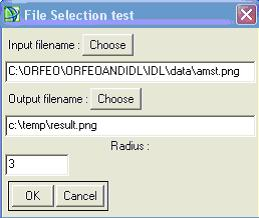
\includegraphics[width=7cm]{fileselectiontest.png}
\caption{File selection}
\end{center}
\end{figure}


\emph{\textbf{Example:}}\\
\indent This is the source code for \emph{simpleENVIGUI.pro} file:\\
\begin{scriptsize}
\indent PRO simpleENVIGUI, ev\\
\\
\indent ; Error handler :\\
\indent err = 0\\
\indent CATCH, err\\
\indent IF err NE 0 THEN BEGIN\\
\indent \indent res = DIALOG\_MESSAGE(!error\_state.msg, /ERROR)\\
\indent \indent res = DIALOG\_MESSAGE(!error\_state.msg, /ERROR)\\
\indent \indent CATCH, /CANCEL\\
\indent \indent RETURN\\
\indent END\\
\\
\indent ; Create simple widgets :\\
\indent base = WIDGET\_AUTO\_BASE(TITLE = 'File Selection test')\\
\\
\indent ; Select input file :\\
\indent wi = WIDGET\_OUTF(base, UVALUE = 'inf', /AUTO, PROMPT = 'Input filename :')\\
\\
\indent ; Select output file :\\
\indent wo = WIDGET\_OUTF(base, UVALUE = 'outf', /AUTO, PROMPT = 'Output filename :', \$\\
\indent DEFAULT = 'c:/temp/result.png')\\
\\
\indent ; Define radius :\\
\indent wRadius = WIDGET\_PARAM(base, DT = 2, PROMPT = "Radius :", /AUTO, UVALUE = "Radius",  DEFAULT = 3)\\
\\
\indent ; Auto manage :\\
\indent result = AUTO\_WID\_MNG(base)\\
\\
\indent ; User hit Cancel button :\\
\indent IF result.accept EQ 0 THEN \$\\
\indent \indent RETURN\\
\\
\indent ; Check values :\\
\indent IF ~FILE\_TEST(result.inf) THEN \$\\
\indent \indent MESSAGE, "Invalid input filename"\\
\indent IF result.outf EQ '' THEN \$\\
\indent \indent MESSAGE, "Invalid output filename"\\
\\
\indent ; Get widget values and do processing :\\
\indent WIDGET\_CONTROL, /HOURGLASS\\
\indent ; Call TOUZI edge detector :\\
\indent OTBTOUZIEDGEDETECTOR, result.inf, result.outf, \$\\
\indent FIX(result.radius)\\
\indent WIDGET\_CONTROL, HOURGLASS = 0\\
\\
\indent ; Load files into ENVI :\\
\indent ENVI\_OPEN\_DATA\_FILE, result.inf\\
\indent ENVI\_OPEN\_DATA\_FILE, result.outf\\
\\
\indent END
\end{scriptsize}
\\

\subsection{ENVI+IDL approach}
In the example below, the GUI is developed using ENVI and IDL widgets. The widgets come from the IDL standard widget library, 
but the loading of the images into ENVI is performed using ENVI routines.

The GUI should look like the figure ~\ref{simpleidlgui}, page~\pageref{simpleidlgui}.
\\
\\
\begin{figure}
\label{simpleidlgui}
\begin{center}
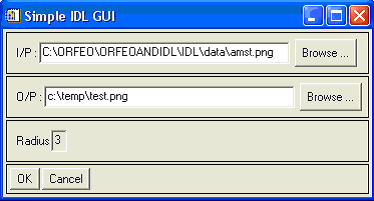
\includegraphics[width=7cm]{simpleidlgui.png}
\caption{Simple IDL GUI}
\end{center}
\end{figure}

The source code contains two main routines:
\begin{itemize}
    \item The � simpleIDLGUI � routine actually builds the GUI.
    \item The � simpleIDLGUI\_event � routine allows handling user events, i.e. to process all user interactions.
    \item The processing itself is performed when the user hits the � OK � button. The � OTBTOUZIEDGEDETECTOR � routine is then called, while passing to it the required parameters.
    \item The loading of the data into ENVI is made by the � ENVI\_OPEN\_DATA\_FILE � routine.
\end{itemize}

\emph{\textbf{Example:}}\\
\indent This is the source code for \emph{simpleIDLGUI.pro} file:\\
\begin{scriptsize}
\indent ; Main event handler :\\
\indent PRO simpleIDLGUI\_event, ev\\
\\
\indent ; Error handler :\\
\indent err = 0\\
\indent CATCH, err\\
\indent IF err NE 0 THEN BEGIN\\
\indent \indent res = DIALOG\_MESSAGE(!error\_state.msg, /ERROR)\\
\indent \indent CATCH, /CANCEL\\
\indent \indent RETURN\\
\indent END\\
\\
\indent ; Get state structure :\\
\indent WIDGET\_CONTROL, ev.top, GET\_UVALUE = pState\\
\\
\indent ; Get user value :\\
\indent WIDGET\_CONTROL, ev.id, GET\_UVALUE = uval\\
\\
\indent CASE uval OF\\
\indent \indent "browseinput": BEGIN\\
\indent \indent \indent strInputFile = DIALOG\_PICKFILE()\\
\indent \indent \indent IF ~FILE\_TEST(strInputFile) THEN \$\\
\indent \indent \indent \indent MESSAGE, "Invalid input filename"\\
\indent \indent \indent WIDGET\_CONTROL, (*pState).wInputFile, SET\_VALUE = strInputFile\\
\indent \indent END\\
\indent \indent "browseoutput": BEGIN\\
\indent \indent \indent strOutputFile = DIALOG\_PICKFILE()\\
\indent \indent \indent WIDGET\_CONTROL, (*pState).wOutputFile, SET\_VALUE = strOutputFile\\
\indent \indent END\\
\indent \indent "OK": BEGIN\\
\indent \indent \indent ; Get input filename :\\
\indent \indent \indent WIDGET\_CONTROL, (*pState).wInputFile, GET\_VALUE = strInputFile\\
\indent \indent \indent ; Test it :\\
\indent \indent \indent IF ~FILE\_TEST(strInputFile) THEN \$\\
\indent \indent \indent \indent MESSAGE, "Invalid input filename"\\
\indent \indent \indent ; Store it :\\
\indent \indent \indent (*pState).strInputFile = strInputFile\\
\indent \indent \indent ; Get output filename :\\
\indent \indent \indent WIDGET\_CONTROL, (*pState).wOutputFile, GET\_VALUE = strOutputFile\\
\indent \indent \indent (*pState).strOutputFile = strOutputFile\\
\indent \indent \indent ; Test it :\\
\indent \indent \indent IF strOutputFile EQ '' THEN \$\\
\indent \indent \indent \indent MESSAGE, "Invalid output filename"\\
\indent \indent \indent ; Store it :\\
\indent \indent \indent (*pState).strOutputFile = strOutputFile\\
\indent \indent \indent ; Read radius :\\
\indent \indent \indent WIDGET\_CONTROL, (*pState).wRadius, GET\_VALUE = radius\\
\indent \indent \indent ; Display hourglass :\\
\indent \indent \indent WIDGET\_CONTROL, /HOURGLASS\\
\indent \indent \indent ; Call TOUZI edge detector :\\
\indent \indent \indent OTBTOUZIEDGEDETECTOR, (*pState).strInputFile, \$ (*pState).strOutputFile,radius\\
\indent \indent \indent ; Hide hourglass :\\
\indent \indent \indent WIDGET\_CONTROL, HOURGLASS = 0\\
\indent \indent \indent ; Load files into ENVI :\\
\indent \indent \indent ENVI\_OPEN\_DATA\_FILE, (*pState).strInputFile\\
\indent \indent \indent ENVI\_OPEN\_DATA\_FILE, (*pState).strOutputFile\\
\indent \indent \indent ; Destroy GUI :\\
\indent \indent \indent WIDGET\_CONTROL, ev.top, /DESTROY\\
\indent \indent END\\
\indent \indent "Cancel": WIDGET\_CONTROL, ev.top, /DESTROY\\
\indent \indent ELSE:\\
\indent END\\
\\
\indent END\\
\\
\indent PRO simpleIDLGUICleanup, tlb\\
\indent WIDGET\_CONTROL, tlb, GET\_UVALUE = pState\\
\indent IF PTR\_VALID(pState) THEN \$\\
\indent \indent PTR\_FREE, pState\\
\indent END\\
\indent ; GUI Definition :\\
\indent PRO simpleIDLGUI, ev\\
\indent base = WIDGET\_BASE(/COLUMN, TITLE = "Simple ENVI Interface")\\
\\
\indent ; Input base :\\
\indent baseIn = WIDGET\_BASE(base, /COLUMN, /FRAME)\\
\indent baseInput = WIDGET\_BASE(baseIn, /ROW)\\
\indent wInputFile = CW\_FIELD(baseInput, TITLE = "I/P :", UVALUE = "inputFile", /STRING, \$\\
\indent XSIZE = 40)\\
\indent wInputButton = WIDGET\_BUTTON(baseInput, VALUE = "Browse ...", UVALUE = "browseinput")\\
\\
\indent ; Ouput base :\\
\indent baseOut = WIDGET\_BASE(base, /COLUMN, /FRAME)\\
\indent baseOutput = WIDGET\_BASE(baseOut, /ROW)\\
\indent wOutputFile = CW\_FIELD(baseOutput, TITLE = "O/P :", UVALUE = "outputFile", /STRING, \$\\
\indent XSIZE = 40)\\
\indent wOutputButton = WIDGET\_BUTTON(baseOutput, VALUE = "Browse ...", UVALUE = "browseoutput")\\
\\
\indent ; Epsilon base :\\
\indent baseEps = WIDGET\_BASE(base, /COLUMN, /FRAME)\\
\indent baseEpsilon = WIDGET\_BASE(baseEps, /ROW)\\
\indent wRadius = CW\_FIELD(baseEpsilon, TITLE = "Radius", /INTEGER, VALUE = 3, \$\\
\indent XSIZE = 1)\\
\\
\indent ; OK/Cancel base :\\
\indent okCancelBase = WIDGET\_BASE(base, /ROW, /FRAME)\\
\indent wOK = WIDGET\_BUTTON(okCancelBase, VALUE = "OK", UVALUE = "OK")\\
\indent wCancel = WIDGET\_BUTTON(okCancelBase, VALUE = "Cancel", UVALUE = "Cancel")\\
\\
\indent ; State structure :\\
\indent st = {strInputFile: '', strOutputFile: '', radius: 0, \$\\
\indent wInputFile: wInputFile, wOutputFile: wOutputFile, wRadius: wRadius}\\
\\
\indent ; Display :\\
\indent WIDGET\_CONTROL, base, /REALIZE, SET\_UVALUE = PTR\_NEW(st, /NO\_COPY)\\
\indent XMANAGER, "simpleIDLGUI", base\\
\\
\indent END\\
\end{scriptsize}

\section{Modification of the IDL path in order to include the directory that contains the files simpleIDLGUI.pro et simpleENVIGUI.pro}
\begin{itemize}
    \item The IDL path can be modified from the IDL Preferences window located in File->Preferences. 
    \item From the Path tab, just add the path to the directory that contains the source code files.
\end{itemize}
The IDL preferences window should look like the figure ~\ref{preferences}, page~\pageref{preferences}.

\begin{figure}
\label{preferences}
\begin{center}
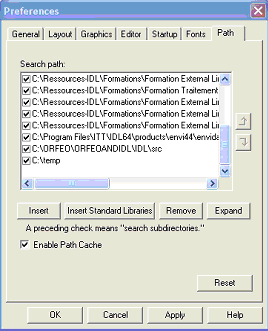
\includegraphics[width=7cm]{preferences.png}
\caption{IDL Prefrences Window}
\end{center}
\end{figure}



\section{Testing from ENVI}
\begin{itemize}
    \item Launch ENVI and select from the main menu bar the ORFEO Filters->Touzi edge detector option.
    \item One of the GUIs simpleENVIGui (see 6.1/) or simpleIDLGui (see 6.2/) will appear depending on the envi.men text file contents (see 2/). 
    \item Select the input and input files. 
    \item Enter a value in the � radius � field and press OK.
    \item The input file as well as the processed image should automatically appear in the ENVI � Available Band List �. 
          They can be displayed in standard ENVI windows(~\ref{bandlist} and ~\ref{viewer}, page~\pageref{bandlist} and page~\pageref{viewer}).
\end{itemize}

\begin{figure}
    \begin{minipage}[b]{.46\linewidth}
        \centering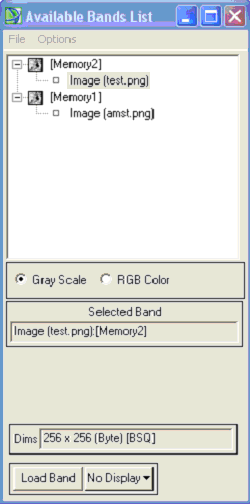
\includegraphics[width=5cm]{bandlist.png}
        \caption{� Available Band List � ENVI window containing input and output image}
        \label{bandlist}
    \end{minipage} \hfill
    \begin{minipage}[b]{.46\linewidth}
        \centering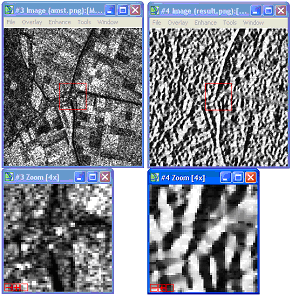
\includegraphics[width=8cm]{viewer.png}
        \caption{Input (left) and Output (right)  examples of a Touzi filter}
        \label{viewer}
    \end{minipage}
\end{figure}

\section{Conclusion}
The integration of OTB routines into ENVI can be done by developing graphical user interfaces, either using only ENVI or using a mixed approach ENVI+IDL. 
The ENVI approach presents lots of advantages :
\begin{itemize}
    \item ENVI widgets are very simple to use, and don't require a deep IDL knowledge.
    \item Source code is very compact.
\end{itemize}

On the other hand, the ENVI+IDL approach is also interesting because it offers a wider widget choice, and allows a deeper widget control.
\\
As a conclusion, the use of the ENVI approach should be fully sufficient in simple cases, whereas The ENVI+IDL approach should be used in more complex situations as drawing images in draw widgets, or using specific widgets not directly available into ENVI.

